\begin{homeworkProblem}[Problem 23.42]

\textbf{A uniform rod of length L and total charge Q lies along the x axis as shown in Figure P23.42. (a) Find the components of the electric field at the point P on the y axis a distance d from the origin. (b) What are the approximate values of the field components when $d >>L$? Explain why you would expect these results.}

Okay, I have a little bit of time so I will try to answer this question in gory detail.

First, I am going to reintroduce the notation I've been emphasizing in this course, so far. For that purpose I am including Figure \ref{fig:vecs.eps} which I included in the document I sent to my ECE 106 tutorial students after Quiz 1. That figure makes it clear how the quantities in which we are interested related. The vector that's of primary importance is $\vec{\scriptr}$ which points from the charge generating the field to the point at which the field is to be evaluated. The two other vectors, $\vec{r}$ and $\vec{r'}$ are used to describe the positions of the point at which we want to calculate the field and the position of the charge, respectively.

Now, we have three vectors and two positions; so, these quantities are not independent. Indeed, $\vec{r'}+\vec{\scriptr} = \vec{r}$. Equivalently, \[\vec{r}-\vec{r'} = \vec{\scriptr} \addtag \]. Okay, now why are these quantities important? Well, they become important when we consider the expression of the electric field due to a point charge: $\vec{E}(\vec{r}) = \frac{k q  \hat{\scriptr}}{|\vec{\scriptr}|^2} = \frac{k q  \vec{\scriptr}}{|\vec{\scriptr}|^3}$ (note that the $\hat{\scriptr}$ changed to a $\vec{\scriptr}$ in the last expression. With a distributed charge problem, it is necessary to integrate over the charge distribution in order to determine the electric fied everywhere in space. This is analogous to how you must sum over the contributions from all discrete charges to find the electric field everywhere in space due to point charges. When we do these integrals, it is very important to keep track of the positions of the charges you are integrating over and the positions at which you want to evaluate the electric field. Note that if we are integrating over a collection of charges which form a charge distribution, we must, by extension, integrate over all the positions at which those charges can exist. This means that we must integrate over $\vec{r'}$ which is responsible for indicating where charge exists. Thus, the problem of finding the electric field due to a line of charge looks like this:

\[ \vec{E}(\vec{r}) = \int_{\text{line of charge}} \frac{k (\vec{r}-\vec{r'}) \diff q'}{|\vec{r}-\vec{r'}|^3} \addtag \]

You should recognize this as the same expression I gave earlier as the electric field due to a point charge. I have just used equation 1 to express $\scriptr$ in terms of $r$ and $r'$. I have also expressed that I will be integrating over the charge. Because that's really what's happening. I'm calculating a portion of the electric field which is due to each infinitesimal chunk of charge that's producing the total field. The positions ($r'$) over which I'm integrating will be determined by the bounds I set up in my integral. So, the integral will define where charge is. $\vec{r}$ is never evaluated until the electric field $\vec{E}(r)$ is evaluated at the point of interest. Thus, this integral over the charge, will involve integrals over $r'$ and, so, $\diff q$ should be expressible in terms of $\vec{r'}$, the coordinate that describes where the charge is located.

How can we determine what $\diff q$ is as a function of $r'$? We need to consider the geometry of the charge distribution. In this case, the charge is distributed along a line. Thus, $\diff q$ can be written as $ \diff q = \lambda \diff l$, where $\lambda$ is the linear charge density. Actually, what's really going on is that $\lambda = \frac{\diff q}{\diff l}$; the charge distribution is found by taking the ratio of the amount of charge in a little chunk of length. If the charge distribution along the line is nonuniform then the amount of charge in a little chunk of length will not be constant - i.e. $\lambda$ will not be a constant. However, in this problem, we are fortunate enough to know that $\lambda$ is a constant as a a function of length.

Now, how does $\diff l$ tie into $r'$ and $r$? Well, $\diff l$ is describing an infinitesimal motion along the path that the charge defines. Our charge distribution, in this problem, is a straight line along the x-axis. Thus, $\diff l = \diff x$. However, because I want to remember that $\diff x$ relates to the position of charges I will label it as $\diff x'$. What are the bounds of my integral? Well, $x'$, the position of my charges, are between 0 and L. Thus, my integration goes from 0 to L. So, my integral is in terms of $x'$. At this point my integral looks like: 

\[ \vec{E}(\vec{r}) = \int_0^L \frac{k (\vec{r}-x'\hat{x}) \lambda \diff x'}{|\vec{r}-x'\hat{x}|^3} \addtag \]

 What is $r'$ in terms of $x'$? Well, $r'$ describes the position of my charges. Thus, while $\vec{r'}$ can in general be expressed as  $ \vec{r'} = x' \hat{x} + y'\hat{y} + z'\hat{z}$, this problem has no charge along the $y$ or $z$ axes so the last two terms can be ignored. Our integral is a function of $\vec{r} = x \hat{x} + y\hat{y} + z\hat{z}$. We can leave it this way. That's fine. Eventually, the problem only wants to know the electric field along the y axis so we can reduce the $\vec{r}$ of interest to $\vec{r} = x\hat{x}$, but that is not necessary. If we wanted to know our electric field along the x or z axes, we could do that, too, at the end. The last thing that we should really do is find a simpler algebraic expression for the denominator of our integrand $|\vec{r}-x'\hat{x}|$. After that, we'll be in a position to solve this integral. 

\begin{align}
    \vec{r} - x'\hat{x} &= x\hat{x} + y\hat{y} + z\hat{z} - x'\hat{x} \nonumber \\
		&= (x - x')\hat{x} + y\hat{y} + z\hat{z} \nonumber \\
		\intertext{What we're interested in is $|\vec{r} - x'\hat{x}|$. But, the magnitude of a vector $\vec{a} = x_a \hat{x} + y_a \hat{y} + z_a \hat{z}$ is $|\vec{a}| = \sqrt{x^2_a + y^2_a + z^2_a}$. Thus:} \nonumber
		|\vec{r} - x'\hat{x}| =& \sqrt{(x-x')^2 + y^2 + z^2} \nonumber
\end{align}

\begin{figure}%
\centering
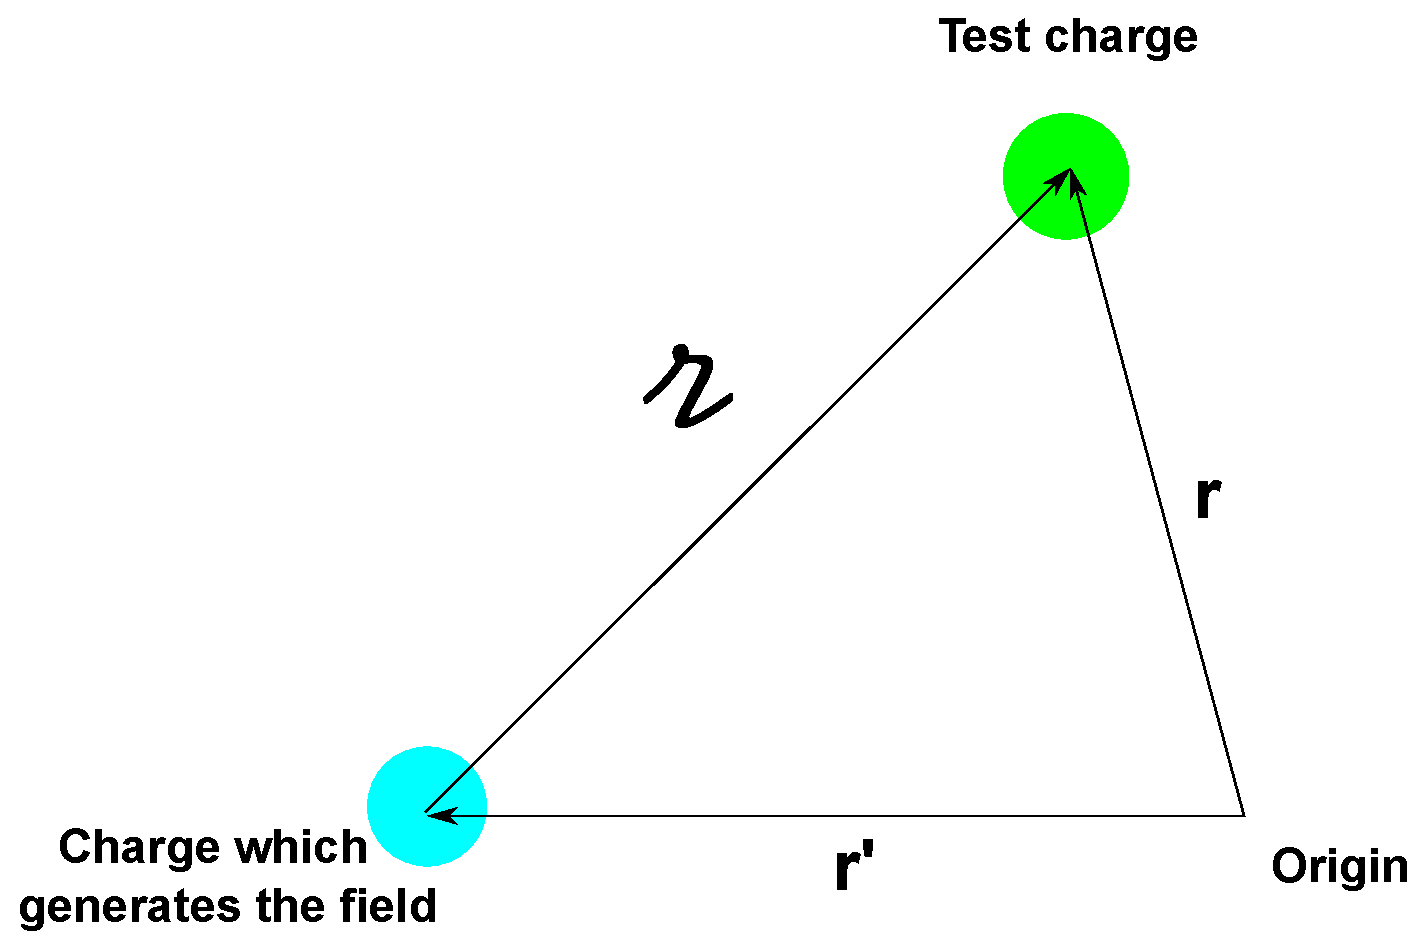
\includegraphics[width=.55\columnwidth]{vecs.eps}%
\caption{Figure used to define the vector convention for this course.}%
\label{fig:vecs.eps}%
\end{figure}

\[ \vec{E}(x,y,z) = \int_0^L \frac{k \big((x-x')\hat{x}+y\hat{y}+z\hat{z}\big) \lambda \diff x'}{\big( x'^2 + y^2\big)^\frac{3}{2}} \addtag \]

This is really three different integrals (all of which can be solved). Since I am only interested in $\vec{E}(0,y,0)$, according to the problem statement, I will set $x$ and $z$ to zero in my integral. If you don't understand why the problem statement restricts $x$ and $z$ to zero remember that we are solving for the electric field only along the y axis and that $x$, $y$ and $z$ (unprimed) are the coordinates where we are evaluating the electric field. Also, note that the solution to the integral for the y axis case looks just like that for the z axis case, which should make sense.

\[ \vec{E}(0,y,0) = \int_0^L \frac{k \big(-x'\hat{x}+y\hat{y} \big) \lambda \diff x'}{\big( x'^2 + y^2\big)^\frac{3}{2}} \addtag \]

Okay, I have everything grouped awkwardly so I'm going to pull out constants and split up the integral into two parts:

\[ \vec{E}(0,y,0) = k \lambda \bigg( \int_0^L \frac{-x'\hat{x} \diff x'}{\big( x'^2 + y^2\big)^\frac{3}{2}} + \int_0^L \frac{y\hat{y} \diff x'}{\big( x'^2 + y^2\big)^\frac{3}{2}} \bigg) \addtag \]

Technically, the $\hat{x}$ and $\hat{y}$ could come out of the integral, too, but it looks a little better, I think, to keep them in. Okay, now this looks a little complicated. However, we are only integrating over $x'$. The y is a constant with respect to the integral. Thus, the first integral looks like: 

\[ \int \frac{x \diff x}{(a^2+x^2)^{1.5}} = -\frac{1}{\sqrt{a^2+x^2}} + C \]

While the second looks like:

\[ \int \frac{\diff x}{(a^2 + x^2)^{1.5}} = \frac{x}{a^2\sqrt{a^2+x^2}} + C\].

I'm pretty sure that you can solve both of these using a u-substitution and turning the crank. I just used Wolfram Alpha. Now, we just have to plug in our bounds and we're done. Doing this yields:


\[ \vec{E}(0,y,0) = k \lambda \bigg( \hat{x} \frac{1}{y^2+x'^2}\Big|_0^L + y \hat{y} \frac{x'}{y^2\sqrt{y^2+x'^2}}\Big|_0^L \bigg) \]

Evaluating these limits:

\[ \vec{E}(0,y,0) = k \lambda \bigg( \hat{x} \big( \frac{1}{\sqrt{L^2+ y^2}} - \frac{1}{y } \big) + \hat{y} \frac{L}{y\sqrt{y^2+L^2}} \bigg) \]

This is the electric field as a function of distance along the y axis (positive and negative). Now, $\lambda$ wasn't given in the problem statement. It's not good to introduce variables for a solution, if avoidable. So, let's substitute $\lambda = \frac{Q}{L}$ since we know that $Q = \lambda L$. 

\[ \vec{E}(0,y,0) = k Q \bigg( \hat{x} \big( \frac{1}{L \sqrt{L^2+ y^2}} - \frac{1}{y L} \big) + \hat{y} \frac{1}{y\sqrt{y^2+L^2}} \bigg) \]

This is the final answer (with $d$ substituted for $y$). When $d$ (or $y$) is much much greater than L (that is: $\frac{L}{d} << 1$) what does the field look like? Well, we need to do the same trick as in the previous problem and Maclaurin expand the electric field about small $\epsilon = \frac{L}{d}$. Recognizing $\frac{L}{y}$ in our radicals in the previous expression, we write:

\[ \vec{E}(0,y,0) = k Q \bigg( \hat{x} \big( \frac{1}{L y\sqrt{(\frac{L}{y})^2+ 1}} - \frac{L}{y L^2} \big) + \hat{y} \frac{1}{y^2 \sqrt{1+(\frac{L}{y})^2}} \bigg) \]

Expressing this in terms of $\epsilon$:

\[ \vec{E}(0,y,0) = k Q \bigg( \hat{x} \big( \frac{\epsilon}{L^2 \sqrt{\epsilon^2+ 1}} - \frac{\epsilon}{L^2} \big) + \hat{y} \frac{\epsilon}{y^2 \sqrt{1+\epsilon^2}} \bigg) \]

I chose to multiply expressions by $ \frac{L}{L}$ instead of $\frac{y}{y}$ because $L$ is a fixed quantity. When I replace $\epsilon$ for $\frac{L}{y}$ want to make sure that I don't eliminate any $y$s. I am going to study the limiting case of large $y$, not small L. By multiplying by $\frac{L}{L}$ I keep the constant $L$, not the variable $y$. Now, performing a Maclaurin series expansion on the first term results in:

\[ \frac{\epsilon}{\sqrt{\epsilon^2+1}} \approx \epsilon - \frac{\epsilon^3}{2} + \cdots \]

The second term does not need to be Maclaurin series expanded. It is already in polynomial form. The last term expands like:

\[ \frac{1}{\sqrt{1+\epsilon^2}} \approx 1 - \epsilon^2/ + \cdots \]

So, finally:

\[ \vec{E}(0,y>>L,0) \approx k Q \bigg( \hat{x} \big( \frac{\epsilon}{L^2} -\frac{\epsilon^3}{2 L^2} - \frac{\epsilon}{L^2} \big) + \frac{\hat{y}}{y^2} \big( 1 - \epsilon^2/2 \big) \bigg) \]

This can be reduced to 

\[ \vec{E}(0,y,0) \approx k Q  \frac{\hat{y}}{y^2} \]

Notice that this just looks like the electric field from a point charge Q located at the origin. This is what the answer to the problem is. 

The way in which you can argue this is that for sufficiently large $y$, $\epsilon$ will be sufficiently small such that terms to higher order than $\epsilon = \frac{L}{y}$ can be ignored. I am not saying that terms of order $\epsilon^3$ don't contribute the electric field. They do. But, if I'm far enough away from the line of charge $\epsilon^3$ looks like nothing. As an example, if my charged length is 1 meter long and I am standing 100 meters away from it $\epsilon^3 = 10^ {-6}$ while $\epsilon = 10^{-2}$. The difference between $\frac{1}{100}$ and $\frac{1}{100.0001}$ is not that large. If you think that's an appreciable difference then I'll stand 1000 meters away. Then $\epsilon^3 = 10^{-9}$ and $\epsilon = 10^{-3}$. The divide between $\epsilon$ and $\epsilon^3$ grew by two orders of magnitude. I could keep doing this.

Okay. I'm done typing now. I hope that this helps.

\end{homeworkProblem}